\documentclass[11pt]{report}
\usepackage{geometry}
\geometry{letterpaper, margin=0.7in}
\usepackage{tgtermes}
\usepackage{graphicx}
\usepackage{verbatim}
\usepackage[spanish]{babel}
\usepackage{subcaption}
\usepackage{subfig} 
\usepackage{multirow}
\usepackage{hyperref}
\usepackage[usenames,dvipsnames,svgnames,table]{xcolor}
\usepackage{ tipa }
\usepackage{ textcomp }
\usepackage{ amssymb }
%%%%%%%%%%%%%%%%%%%%

\begin{document}

\today

Consuelo Dayzu Quinto

\begin{center}
\large \textbf{Concordancia entre genotipos de MEGA (Illumina) y 1KG (Affymetrix)/HapMap (Affymetrix+Illumina)}
\end{center}
\\

A continuacion se muestran los resultados de 3 rondas de analisis de la corrida de entrenamiento del HiScan, con el microarreglo MEGA de Illumina. 

\begin{table}[ht]
\centering
\caption{Muestras usadas en la corrida de entrenamiento}
\label{my-label}
\begin{tabular}{|l|l|}
\hline
\multicolumn{1}{|l|}{ID muestra} & \multicolumn{1}{l|}{Plataforma} \\ \hline \hline
NA21402 & HapMap \\
NA12878 & HapMap/1KG \\
NA21405 & HapMap \\
HG01938 & 1KG \\
NA21685 & HapMap \\
HG01941 & 1KG \\
NA19088 & HapMap/1KG\\ \hline
%%NA21732 & ? \\ \hline
\end{tabular}
\end{table}

Cada ronda de analisis consiste en los siguientes pasos: 
\begin{itemize}
\item Los genotipos fueron generados usando GenomeStudio con el manifiesto 
MEGA\_Consortium\_15063755\_B2, y con las siguientes variaciones:
\begin{enumerate}
\item sin cluster file
\item PAGE cluster file (\url{https://www.pagestudy.org/index.php/multi-ethnic-genotyping-array})
\item GLOBAL cluster file (en la computadora de HiScan: MEGA-Global:multi-ethnic-global-8-cluster-file/Multi-EthnicGlobal\_ClusterFile.egt)
\end{enumerate}

\item SNPs en cromosomas 0, X, Y, XY y MT fueron filtrados, al igual que SNPs con missing call superiores a 0:\\
\colorbox{Lavender}{plink --file [archivo] --geno 0 --not-chr 0,X,Y,XY,MT --recode --out [archivo]}

\item Los identificadores de los SNPs fueron renombrados a rsID usando el archivo
\\ MEGA\_Consortium\_v2\_15070954\_A1\_b138\_rsids.txt.

\item SNPs con el mismo rsID y la misma posicion fisica tambien fueron removidos:\\
\colorbox{Lavender}{plink --file [archivo] --exclude [lista duplicados] --recode --out [archivo]}\\
\colorbox{Lavender}{plink --file [archivo] --list-duplicate-vars}

\item Para cada cluster file usado, se hizo una comparacion con los genotipos obtenidos por 1000 Genomes (1KG) y HapMap:
\begin{enumerate}
\item 1KG: Affymetrix 6.0 (863, 597 SNPs)
\item HapMap3: Illumina Human1M y Affymetrix SNP 6.0 (1, 374, 871 SNPs)
\end{enumerate}

\item Se encontraron los SNPs en comun entre cada una de las plataformas (busqueda por rsID) y se omitieron SNPs que  tuvieran por nombre ``.''.

\item Con plink, se unieron los diferentes sets de datos (entrenamiento+1KG y entrenamiento+HapMap) y se cambiaron las cadenas (AC a TG) para algunas variantes: \\
\colorbox{Lavender}{plink --bfile [archivo1] --bmerge [archivo2.bed/bim/fam] --recode --out [archivo3]}\\
\colorbox{Lavender}{plink --bfile [archivo2] --flip [archivo2.missnp] --make-bed -out [archivo2]}\\
\colorbox{Lavender}{plink --bfile [archivo1] --bmerge [archivo2.bed/bim/fam] --recode --out [archivo3]}

\item Para comparar los genotipos de los mismos individuos en las diferentes plataformas, se uso el script cal\_concordance.pl, el cual compara los genotipos y calcula el numero de diferencias:\\
\colorbox{Lavender}{\$matches = (\$split1[1] \textasciicircum   \$split2[1]) =$\sim$ tr \textfractionsolidus \textbackslash 0 \textfractionsolidus \textfractionsolidus;} 
\end{itemize}

En la siguiente tabla estan los resultados de concordancia entre los diferentes analisis:  
\begin{table}[ht]
\centering
\label{my-label}
\begin{tabular}{|l|l|l|l||l|l|l|}
\hline \hline
\multirow{2}{*}{} & \multicolumn{3}{c|}{Concordancia con HapMap} & \multicolumn{3}{c|}{Concordancia con 1KG} \\ \cline{2-7} 
 & No cluster & cluster PAGE & cluster GLOBAL & No cluster & cluster PAGE & cluster GLOBAL \\ \hline \hline
\begin{tabular}[c]{@{}l@{}}\% concordancia\\ (promedio)\end{tabular} & 96\% & 94\% & 94\% & 94\% & 92\% & 92\% \\ \hline
\# SNPs & 282, 831 & 279, 879 & 268, 907 & 128, 587 & 127, 318 & 122, 581 \\ \hline
\end{tabular}
\end{table}

En las siguientes figuras se muestran los porcentajes de concordancia (en naranja) entre los genotipos de los individuos en la corrida de entrenamiento, en 1KG y en HapMap. 

\begin{figure}[ht]
    \centering
    \caption{Comparacion sin cluster}
    \begin{subfigure}[t]{0.5\textwidth}
        \centering
        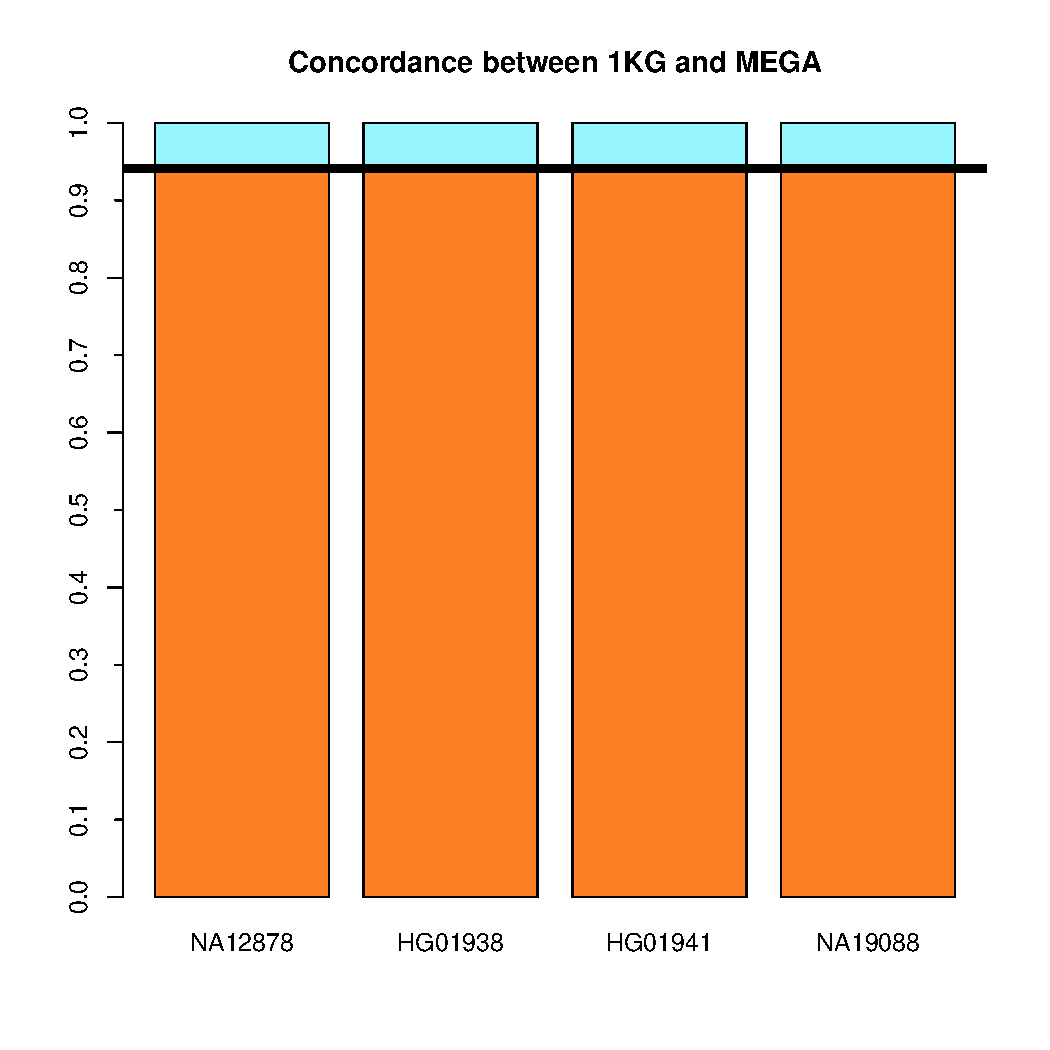
\includegraphics[scale=0.55]{Concordance_1KG_MEGA_nocluster.pdf}
    \end{subfigure}%
    ~ 
    \begin{subfigure}[t]{0.5\textwidth}
        \centering
        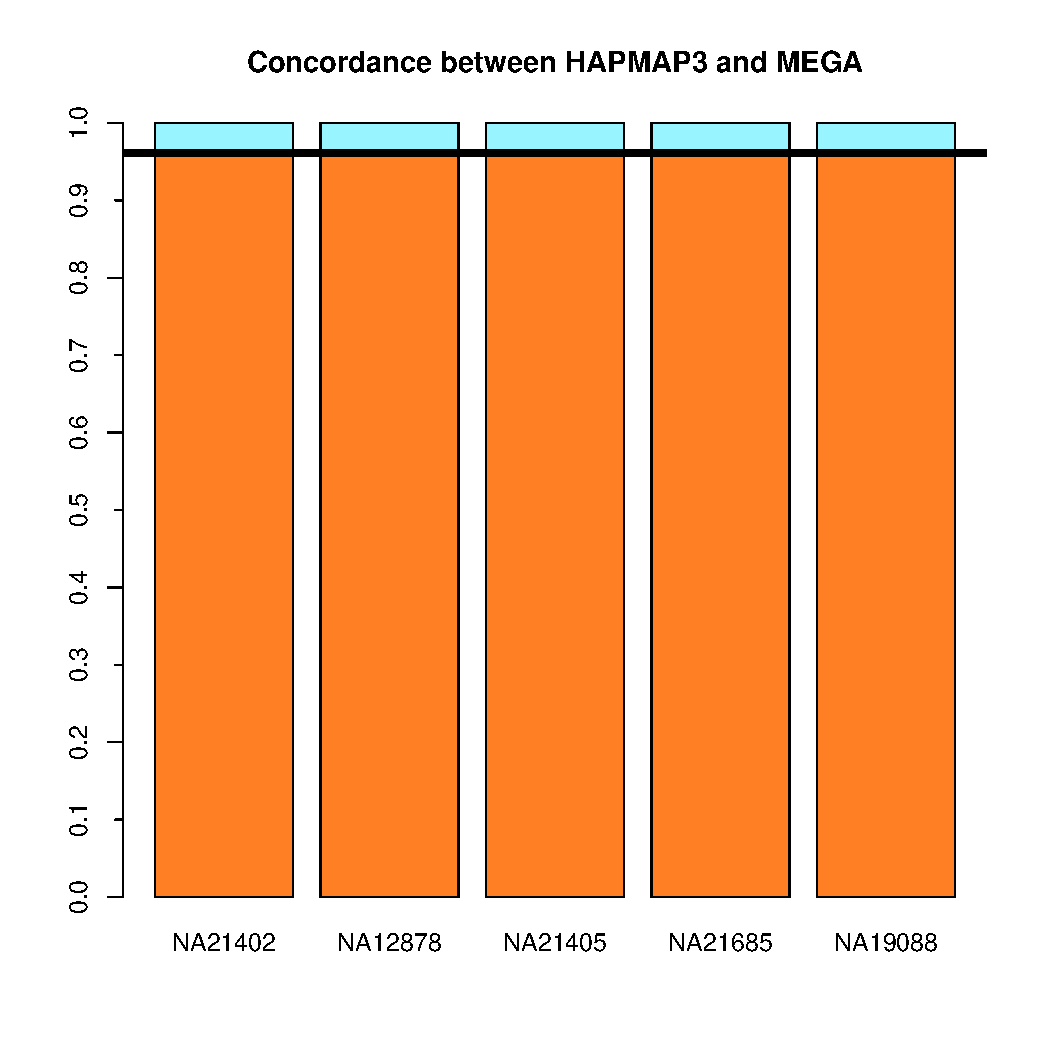
\includegraphics[scale=0.55]{Concordance_HAPMAP_MEGA_nocluster.pdf}
	 \end{subfigure}
\end{figure}

\newpage
%%%%%%%%%%%%%%%
\begin{figure}[ht!]
    \centering
    \caption{Comparacion cluster PAGE}
    \begin{subfigure}[t]{0.5\textwidth}
        \centering
        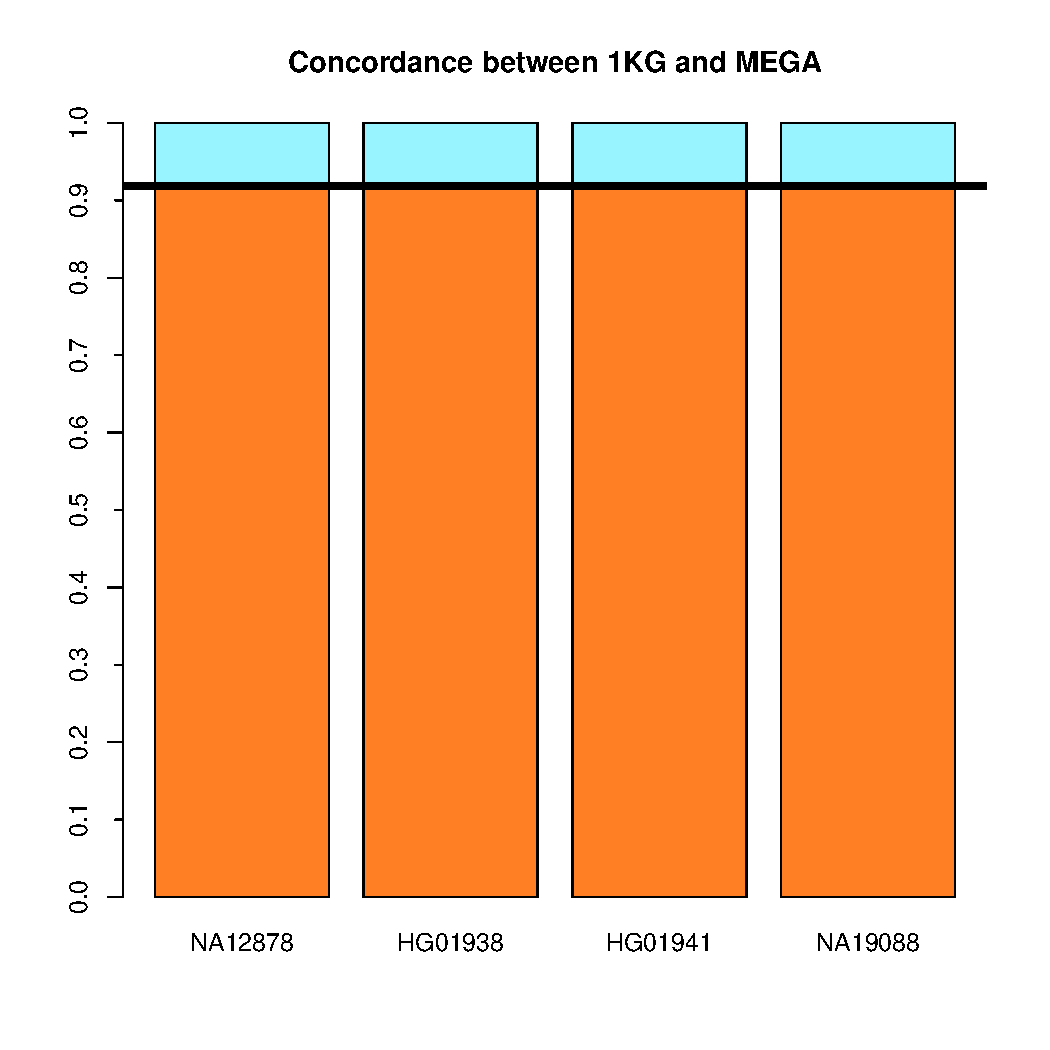
\includegraphics[scale=0.55]{Concordance_1KG_MEGA_clusterPAGE.pdf}
    \end{subfigure}%
    ~ 
    \begin{subfigure}[t]{0.5\textwidth}
        \centering
        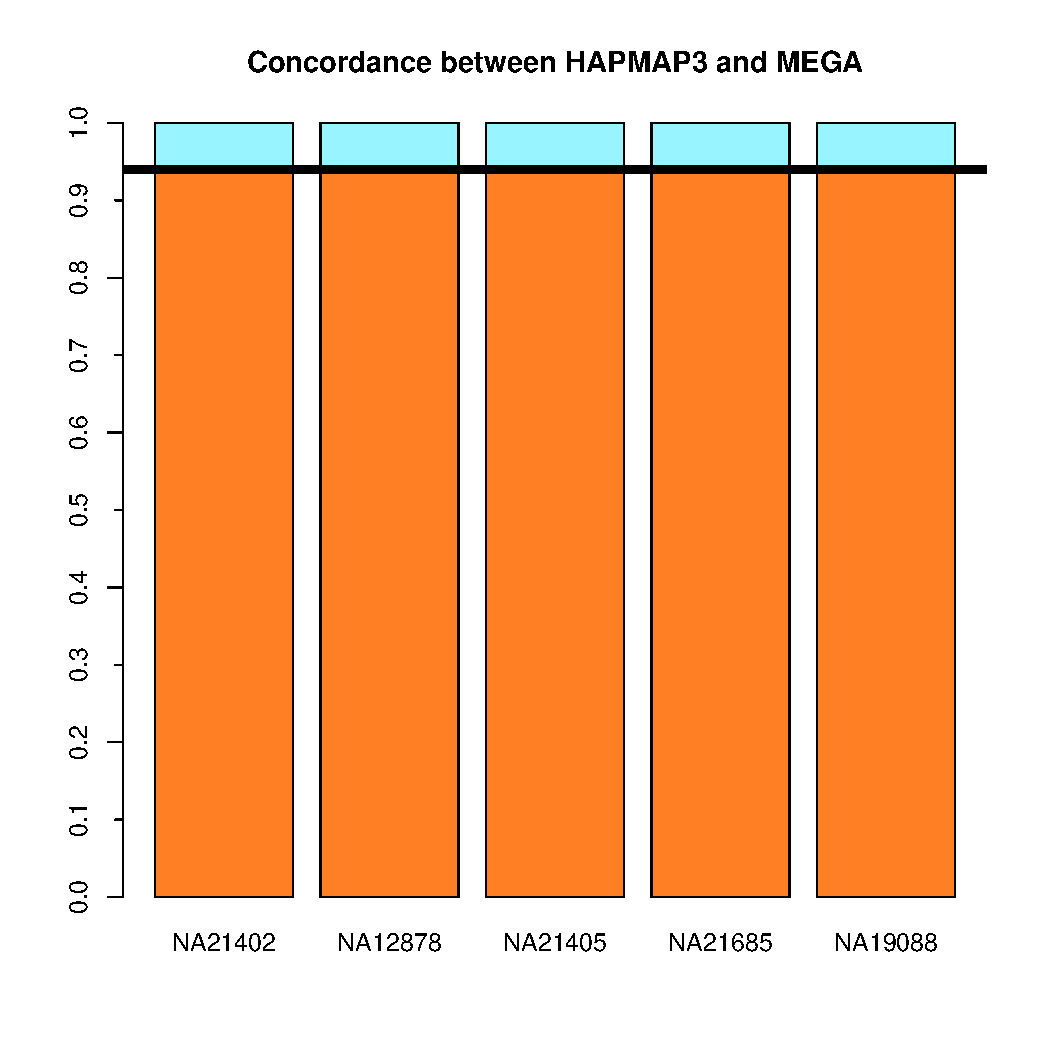
\includegraphics[scale=0.55]{Concordance_HAPMAP_MEGA_clusterPAGE.pdf}
    \end{subfigure}
\end{figure}

\newpage
%%%%%%%%%%%%%%%
\begin{figure}[ht!]
    \centering
    \caption{Comparacion cluster GLOBAL}
    \begin{subfigure}[t]{0.5\textwidth}
        \centering
        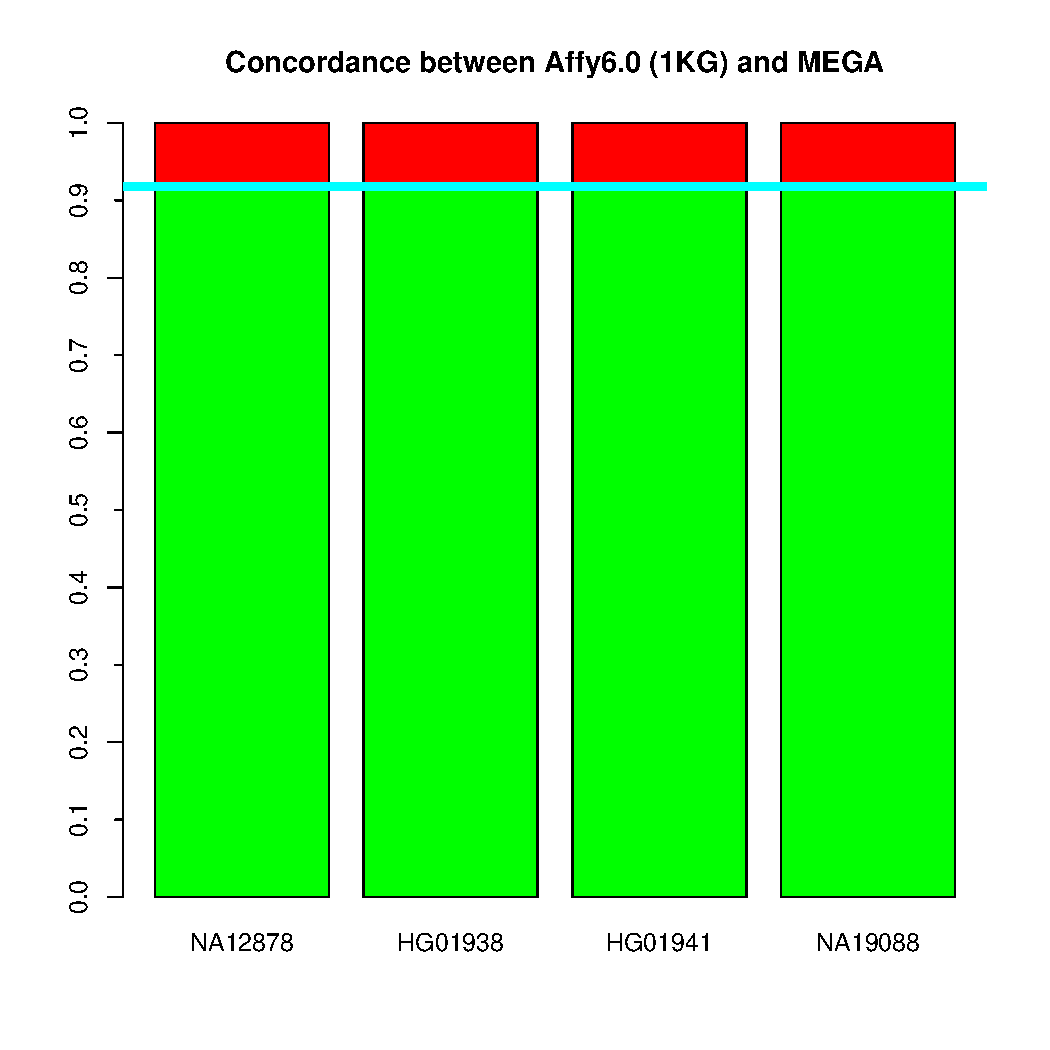
\includegraphics[scale=0.55]{Concordance_1KG_MEGA_clusterGLOBAL.pdf}
    \end{subfigure}%
    ~ 
    \begin{subfigure}[t]{0.5\textwidth}
        \centering
        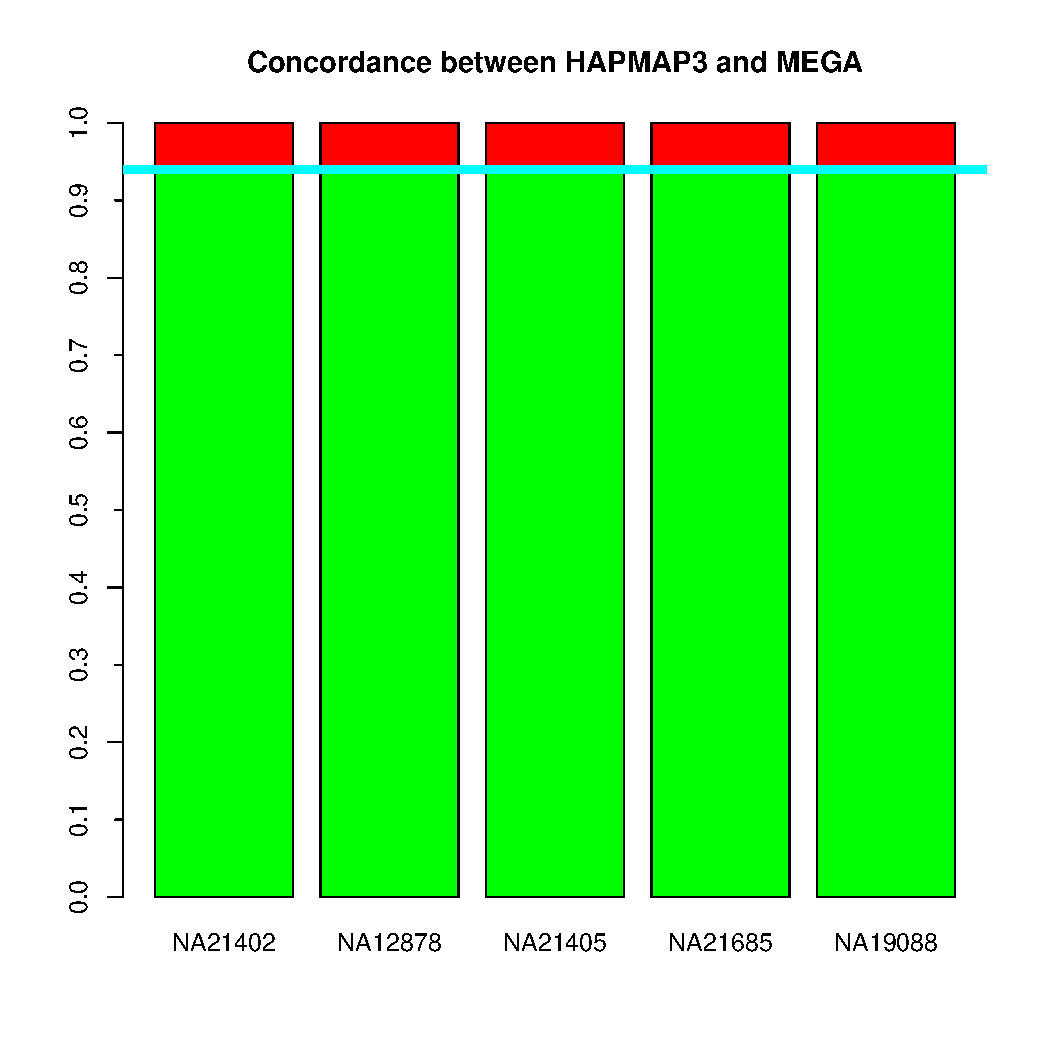
\includegraphics[scale=0.55]{Concordance_HAPMAP_MEGA_clusterGLOBAL.pdf}
    \end{subfigure}
\end{figure}

\textit{(Los archivos README* tienen mas informacion acerca de los pasos que se siguieron para renombrar los SNPs, filtrar y unir los datos.)}

\newpage

En base al analisis realizado en el primer batch de muestras de Maria Avila y 1KG, me di cuenta que hay sitios que tienen, por ejemplo, un genotipo CC, mientras que en el segundo set de datos, el mismo genotipo es GG (lo mismo aplica para genotipos AA y TT). Con el script cal\_concordance2.pl, se tomaron en cuenta este tipo de sitios y los nuevos porcentajes de concordancia estan el siguiente tabla: \\
\begin{table}[ht]
\centering
\label{my-label}
\begin{tabular}{|l|l|l|l||l|l|l|}
\hline \hline
\multirow{2}{*}{} & \multicolumn{3}{c|}{Concordancia con HapMap} & \multicolumn{3}{c|}{Concordancia con 1KG} \\ \cline{2-7} 
 & No cluster & cluster PAGE & cluster GLOBAL & No cluster & cluster PAGE & cluster GLOBAL \\ \hline \hline
\begin{tabular}[c]{@{}l@{}}\% concordancia\\ (promedio)\end{tabular} & 99.81\% & 99.96\% & 99.96\% & 99.82\% & 99.97\% & 99.98\% \\ \hline
\# SNPs & 282, 831 & 279, 879 & 268, 907 & 128, 587 & 127, 318 & 122, 581 \\ \hline
\end{tabular}
\end{table}

%%%%%%%%%%%%%%%%%%%%%%%%%%%

\begin{center}
\large \textbf{GenomeStudio e informacion acerca de la posicion de los SNPs (cadena positiva/negativa)}
\end{center}
\\

En las corridas de analisis de Genome Studio con las muestras del entrenamiento y usando el manifiesto \\ MEGA\_Consortium\_15063755\_B2.bpm, no se muestra en la SNP Table la informacion acerca de la cadena donde se encuentran los SNPs (+ vs -). \\

Sin embargo, esta informacion si aparece cuando se analizaron las muestras de Maria Avila con el microarreglo de MEGA comercial y el manifiesto Multi-EthnicGlobal\_A1.bpm. A pesar de esto, parece que la informacion de la direccion de las cadenas no se transmite a plink, ya que los archivos creados por el plugin de plink siguen teniendo alelos en la cadena - (TT vs AA). \\ 

Ejemplo: \\
rsId: rs2465136\\
posicion: 1: 990417\\
muestra: HG01938 (1KG)\\
\\
Informacion de dbSNP: A/G (REV)\\
Alelos en 1KG: TT \\
Alelos en MEGA reportados por GenomeStudio: AA \\

Algo que se puede hacer para encontrar sitios donde esto ocurre es generar un reporte final desde GenomeStudio donde se encuentra la informacion acerca de la direccion de las cadenas (Plus/Minus Strand), pero solo usando el manifiesto Multi-EthnicGlobal\_A1.bpm. 

Una sugerencia de Pavel es generar una lista de SNPs (basada en el reporte final) donde potencialmente habria un problema de cadena + vs. cadena -, para que el usuario sepa que esos alelos se tienen que cambiar con plink (\colorbox{Lavender}{opcion --flip lista.txt}) cuando se querian unir varios sets de datos como 1KG y/o HapMap. 

\end{document}

